\documentclass[12pt,a4paper,twoside,openright,titlepage,final]{article}
\usepackage{fontspec}
\usepackage{amsmath}
\usepackage{amsfonts}
\usepackage{amssymb}
\usepackage{makeidx}
\usepackage{graphicx}
\usepackage[hidelinks,unicode=true]{hyperref}
\usepackage[spanish,es-nodecimaldot,es-lcroman,es-tabla,es-noshorthands]{babel}
\usepackage[left=3cm,right=2cm, bottom=4cm]{geometry}
\usepackage{natbib}
\usepackage{microtype}
\usepackage{ifdraft}
\usepackage[obeyDraft]{todonotes}
\ifdraft{
	\usepackage{draftwatermark}
	\SetWatermarkText{BORRADOR}
	\SetWatermarkScale{0.7}
	\SetWatermarkColor{red}
}{}
\usepackage{booktabs}
\usepackage{longtable}
\usepackage{calc}
\usepackage{array}
\usepackage{caption}
\usepackage{subfigure}
\usepackage{footnote}
\usepackage{url}
\setsansfont[Ligatures=TeX]{texgyreadventor}
\setmainfont[Ligatures=TeX]{texgyrepagella}

%*******************************************************
%                 NO MODIFICAR
\newcommand*{\FSfont}[1]{%
  \fontencoding{T1}\fontfamily{#1}\selectfont}

\newlength{\tpheight}\setlength{\tpheight}{0.9\textheight}
\newlength{\txtheight}\setlength{\txtheight}{0.9\tpheight}
\newlength{\tpwidth}\setlength{\tpwidth}{0.9\textwidth}
\newlength{\txtwidth}\setlength{\txtwidth}{0.9\tpwidth}
\newlength{\drop}
%*******************************************************

% Crea una portada con los siguientes parámetros
%
% #1 : Título 
% #2 : Subtítulo
% #3 : Subsubtítulo
% #4 : Autor(es)
% #5 : Lugar
%

\newcommand*{\portada}[5]{
\begin{titlepage}
\begingroup
\vspace*{1cm}
\drop = 0.2\txtheight
\centering
\vfill
{\Huge \scshape #1}\\[\baselineskip]
{\Large \textbf{#2}}\\[\baselineskip]
{\Large \scshape #3}\\[\baselineskip]
\vspace*{0.3cm}
{\large \textit{#4}}\\[0.5\drop]

\includegraphics[scale=0.35]{./imagenes/logoURJC.jpg}
\vspace*{1.5cm}

{\large \scshape #5, \today} \par
\begin{center}
\end{center}
\vfill\null
\endgroup
\end{titlepage}
}
 %*****************************************************
 


\author{José Ignacio Escribano}

\title{Caso práctico I}

\setlength{\parindent}{0pt}

\begin{document}

\pagenumbering{alph}
\setcounter{page}{1}

\portada{Caso Práctico I}{Modelización y tratamiento de la incertidumbre}{Estadística descriptiva}{José Ignacio Escribano}{Móstoles}

\listoffigures
\thispagestyle{empty}
\newpage

\tableofcontents
\thispagestyle{empty}
\newpage


\pagenumbering{arabic}
\setcounter{page}{1}

\section{Introducción}

Para la realización de este caso práctico requerimos dos conjuntos de datos: un conjunto cuantitativo discreto y otro cuantitativo continuo. Cuando dispongamos de estos conjuntos de datos procederemos a realizar un análisis descriptivo de cada uno éstos.\\

Para ello, necesitamos encontrar una base de datos que disponga de los conjuntos de datos requeridos anteriormente. La base de datos elegida se centra en el estudio de la liga norteamericana de béisbol de la temporada 1986. Los datos se encuentran disponibles en el siguiente enlace: \url{http://lib.stat.cmu.edu/datasets/baseball.data}\footnote{El archivo se encuentra en forma de ``shell archive'', que es una forma de fichero autoextraíble, en el que se agrupan varios archivos, tanto de datos como descripciones de las variables. Para poder extraer estos ficheros, ejecutaremos en una terminal el comando \textbf{sh} seguido del nombre del fichero. Esto creará cuatro ficheros: \textit{pitcher.final}, \textit{team.final}, \textit{data.des.form}, \textit{hitter.final}. De estos ficheros sólo nos interesan los dos últimos: en el primero se encuentran las descripciones de las variables; y en el segundo, los datos que utilizaremos para nuestro análisis descriptivo.}. En el archivo se encuentran distintos datos relativos a equipos, pitchers y hitters. Nos centraremos en estos últimos. De entre las $24$ variables disponibles en el fichero utilizaremos como variable cuantitativa discreta el número de homeruns durante la temporada 1986, y como variable cuantitativa continua el salario al comienzo de la temporada 1987.  

\section{Análisis descriptivo de un conjunto de datos cuantitativos discretos}

El conjunto de datos cuantitativo discreto elegido es \textbf{el número de homeruns de los ``hitters'' de la liga norteamericana de béisbol durante la temporada 1986}.\\

Para realizar el análisis descriptivo de este conjunto de datos, realizaremos distintos tipos de gráficos como el gráfico de barras y sectores, entre otros. Posteriormente, daremos una serie de medidas, tanto de centralización, posición como dispersión.\\

Comencemos realizando el diagrama de barras para ver como se distribuye la frecuencia de cada uno de los posibles valores de la variable número de homeruns. En la Figura~\ref{fig:diagrama_barras_homeruns} se muestra este diagrama. Se puede observar que la frecuencia se mantiene más o menos constante entre los $0$ y $9$ homeruns, mientras que a partir de $10$, la frecuencia desciende de manera considerable. Y la realización de $31$ homeruns o más es bastante infrecuente.\\

\begin{figure}[tbph!]
\centering
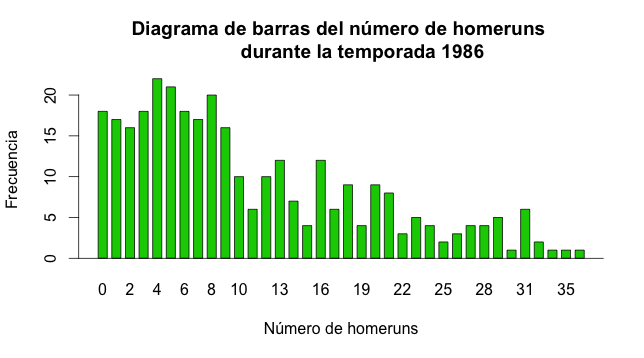
\includegraphics[width=0.8\linewidth]{imagenes/diagrama_barras_homeruns}
\caption{Diagrama de barras para el número de homeruns}
\label{fig:diagrama_barras_homeruns}
\end{figure}

Si realizamos el diagrama de sectores (Figura~\ref{fig:diagrama_sector_homeruns}), veremos que el número de posibles valores es $41$: desde $0$ hasta $40$ homeruns, que es el máximo. Debido a este gran número de valores, el gráfico no se aprecia bien.\\

\begin{figure}[tbph!]
\centering
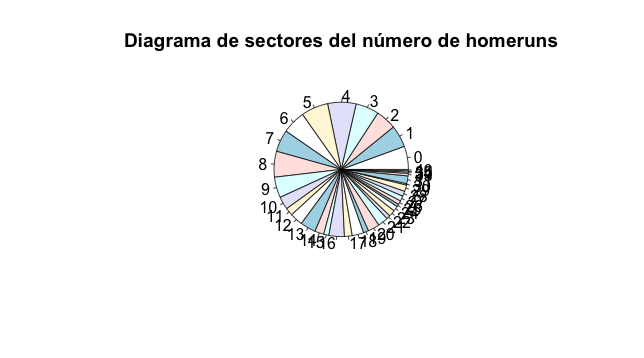
\includegraphics[width=0.8\linewidth]{imagenes/diagrama_sectores_homeruns}
\caption{Diagrama de sectores para el número de homeruns}
\label{fig:diagrama_sector_homeruns}
\end{figure}

Para asegurarnos de que lo visto en los gráficos anteriores se corresponde con la realidad de los datos, calcualremos una serie de medidas de distintos tipos: de centralización, de posición y de dispersión. \\

Las medidas de centralización que consideraremos son la media aritmética, la mediana y la moda. Estas medidas son:

\begin{table}[htbp]
\centering
\begin{tabular}{|c|c|}
\hline Media & 10.77019 \\ 
\hline Mediana & 8 \\ 
\hline Moda & 10  \\ 
\hline 
\end{tabular} 
\end{table}

Como estas medidas son más o menos similares, podemos decir que estas medidas son bastante representativas de estos datos.\\


Las medidas de posición que consideraremos serán los cuartiles y los deciles. Entre los primeros, optaremos por el primer ($Q_1$) y el tercer cuartil ($Q_3$); y de los segundos, optaremos por el segundo ($D_2$) y el noveno decil ($D_{9}$). \\

\begin{table}[htbp]
\centering
\begin{tabular}{|c|c|}
\hline $Q_1$ & 4 \\ 
\hline $Q_3$ & 16 \\ 
\hline $D_2$& 3  \\ 
\hline $D_9$& 24  \\ 
\hline 
\end{tabular} 
\end{table}

De los cuartiles $Q_1$ y $Q_3$ concluimos que el $25\%$ de los jugadores consiguen $4$ o menos homeruns y que el $75 \%$ es menor o igual a $16$. De la misma forma, el $20\%$ de los jugadores consiguen menos de $3$ homeruns; y el $90\%$ hace $24$ o menos homeruns.\\

Las medidas de dispersión son la varianza y la cuasivarianza, la desviación estándar, el rango y el rango intercuartílico.\\

\begin{table}[htbp]
\centering
\begin{tabular}{|c|c|}
\hline Varianza & 75.61178 \\ 
\hline Cuasivarianza & 75.84733 \\
\hline Desviación estándar & 8.709037 \\  
\hline Rango & 40  \\ 
\hline Rango intercuartílico & 12  \\ 
\hline 
\end{tabular} 
\end{table}

De los resultados anteriores vemos que la varianza es muy elevada, lo que hace haya gran variabilidad de los datos. El rango también es muy grande debido a todos los posibles valores que toman los datos: entre $0$ y $40$.\\

Con el rango intercuartílico podemos obtener el diagrama de cajas (Figura~\ref{fig:diagrama_cajas_homeruns}). Podemos observar que el rango intercuartílico se sitúa entre $4$ y $16$ homeruns y la mediana es de $8$ homeruns. Hay que destacar que hay dos datos atípicos, por lo que conseguir $35$ ó $40$ homeruns es poco común en los jugadores de la temporada 1986.  

\begin{figure}[tbph!]
\centering
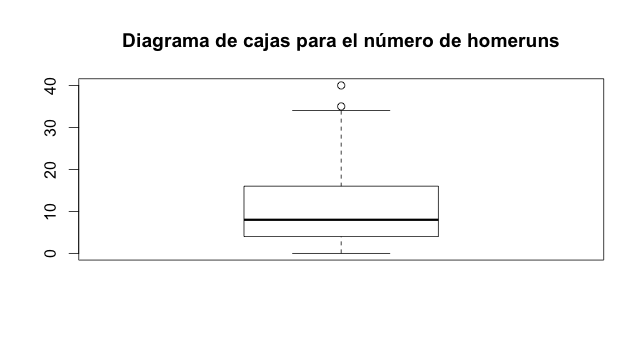
\includegraphics[width=0.8\linewidth]{imagenes/diagrama_cajas_homeruns}
\caption{Diagrama de cajas para el número de homeruns}
\label{fig:diagrama_cajas_homeruns}
\end{figure}

\section{Análisis descriptivo de un conjunto de datos cuantitativos continuos}

\end{document}